\documentclass[12pt]{article}
\usepackage[a4paper, margin=2cm]{geometry}
\usepackage{parskip}
\usepackage[dvipsnames]{xcolor}

\usepackage{amsmath}
\usepackage{amssymb}
\usepackage{enumitem}
\usepackage{fancyhdr}
\usepackage{float}
\usepackage{helvet}
\usepackage{hyperref}
\usepackage{graphicx}

\renewcommand{\familydefault}{\sfdefault}
\setlength{\parindent}{0}

\begin{document}

    \title{PiRover}

    \date{}
    \author{
        k12008656, Abdu`llah Arij\\
        k12223453, Olivotto Philipp\\
        k12315349, Pichler Alexander\\
        k12308997, Schoenberger Fabian\\
        k12309011, Siala Alexander
    }

    \maketitle
    \tableofcontents

    \section*{Contribution Table}
    \begin{flushleft}
        \begin{minipage}{0.6\textwidth}
            \begin{table}[H]
                \centering
                \renewcommand{\arraystretch}{1.3}
                \begin{tabular}{|l|p{7.5cm}|}
                    \hline
                    \textbf{Task} & \textbf{Contributors} \\
                    \hline
                    Rover & Schönberger Fabian, Siala Alexander \\
                    Web Interface & Pichler Alexander, Abdu`llah Arij  \\
                    Grafana & Olivotto Philipp \\
                    Report & Everyone \\
                    Presentation &  Siala Alexander \\
                    Video & Schönberger Fabian \\
                    \hline
                \end{tabular}\label{tab:table}
            \end{table}
        \end{minipage}
    \end{flushleft}

    \newpage

    \section{Description / Introduction}

Our project is based on the Freenove Three-Wheeled Smart Car Kit for Raspberry Pi. We use the hardware from the kit and follow the tutorial as a starting point, but we develop our own custom software to control the vehicle.
The kit includes a car frame, two wheels for steering and driving, a buzzer, an RGB light, a camera, and all necessary parts like screws and cables. It also comes with a special shield to control everything via a Raspberry Pi.

In addition, we use two lithium-ion batteries for power and a Raspberry Pi 4 to control the car.

We call our vehicle PiRover. It can be controlled through a Svelte-based web user interface. Communication with the PiRover works over Wi-Fi using MQTT and WebSockets. This allows us to send commands and receive data in real time.
Additionally, the camera’s live video feed is streamed to the web interface, allowing users to see the rover’s point of view.


\begin{figure}[h!]
    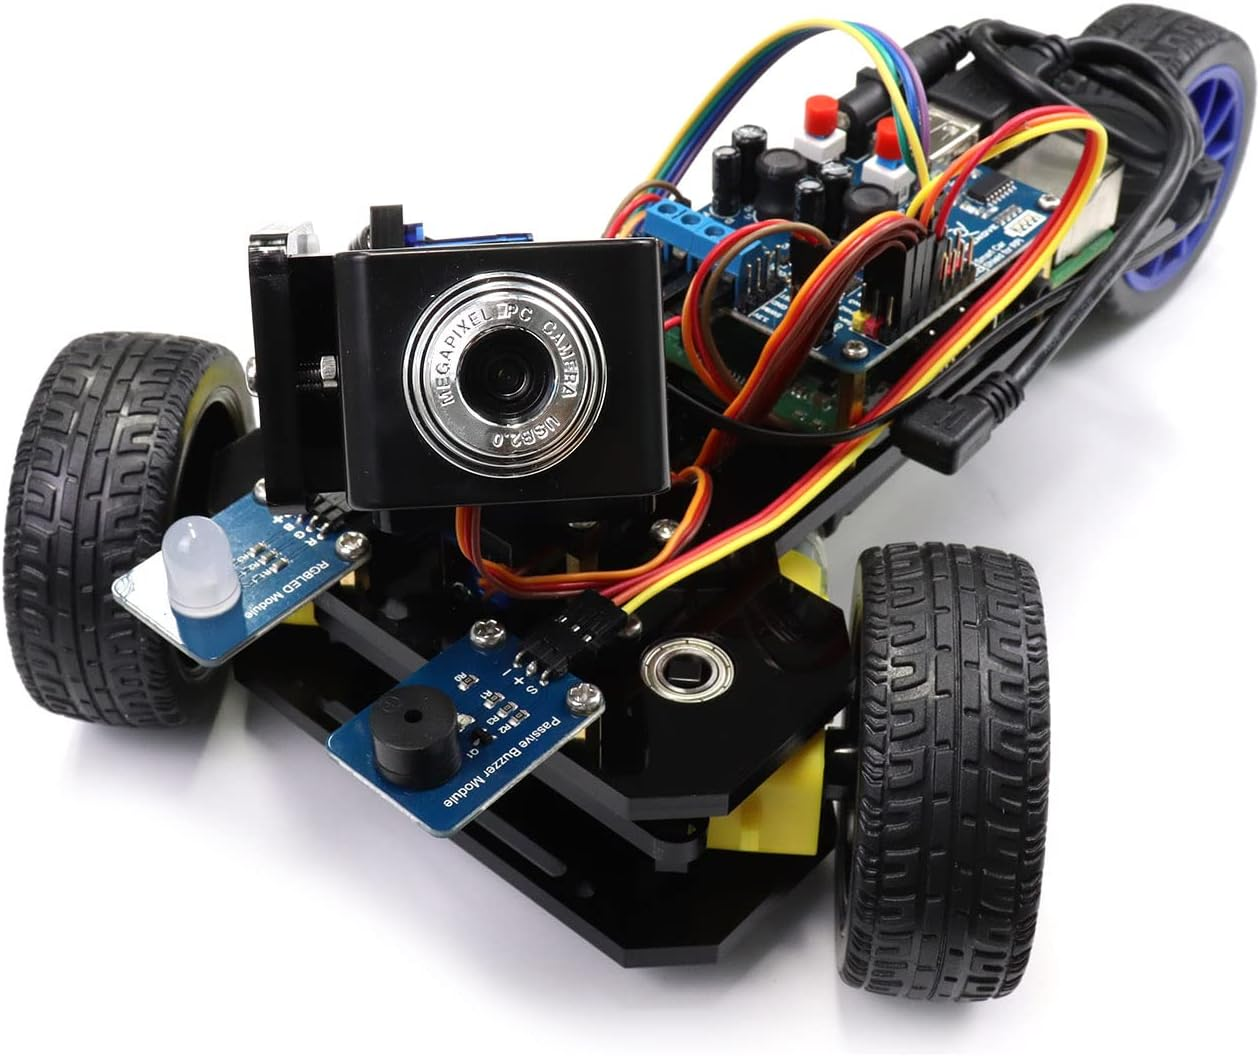
\includegraphics[width=15cm]{img/freenove_smartcar_imagepicture}
\end{figure}

    \section{Architecture}

%TODO Add project architecture (UML, SysUMl,...)

The rover itself consists of a python script that controls the hardware, provides a websocket for the camera feed and controls, and publishes sensor and actuator data to MQTT.
Another python script subscribes to this data from the rover and inserts it into a postgres database, which is then accessed by a Grafana dashboard (also running on the RPi).
Lastly, the browser accesses our web interface (which is running locally on the user's device for now), and establishes a websocket connection with the rover.

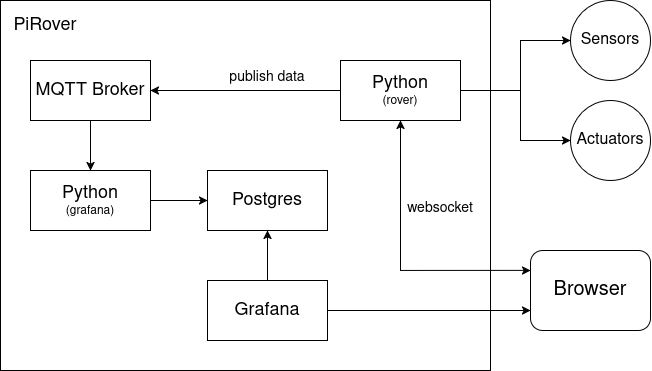
\includegraphics[width=0.8\textwidth]{img/architecture}

    \section{Rover}

%TODO List the following infos about the rover:
%Software
%Communication protocols
%Sensors/actuators
%Users and user stories


\subsection{Setup}
\subsubsection{Hardware}
\subsubsection{Software}
\subsubsection{Testing}


\subsection{Software}









    \section{Web}

The software in the \texttt{web/} folder is a svelte web application that allows the user to connect to PiRover, view the live camera feed and control the Rover. An image follows:

\begin{figure}[H]
    \centering
    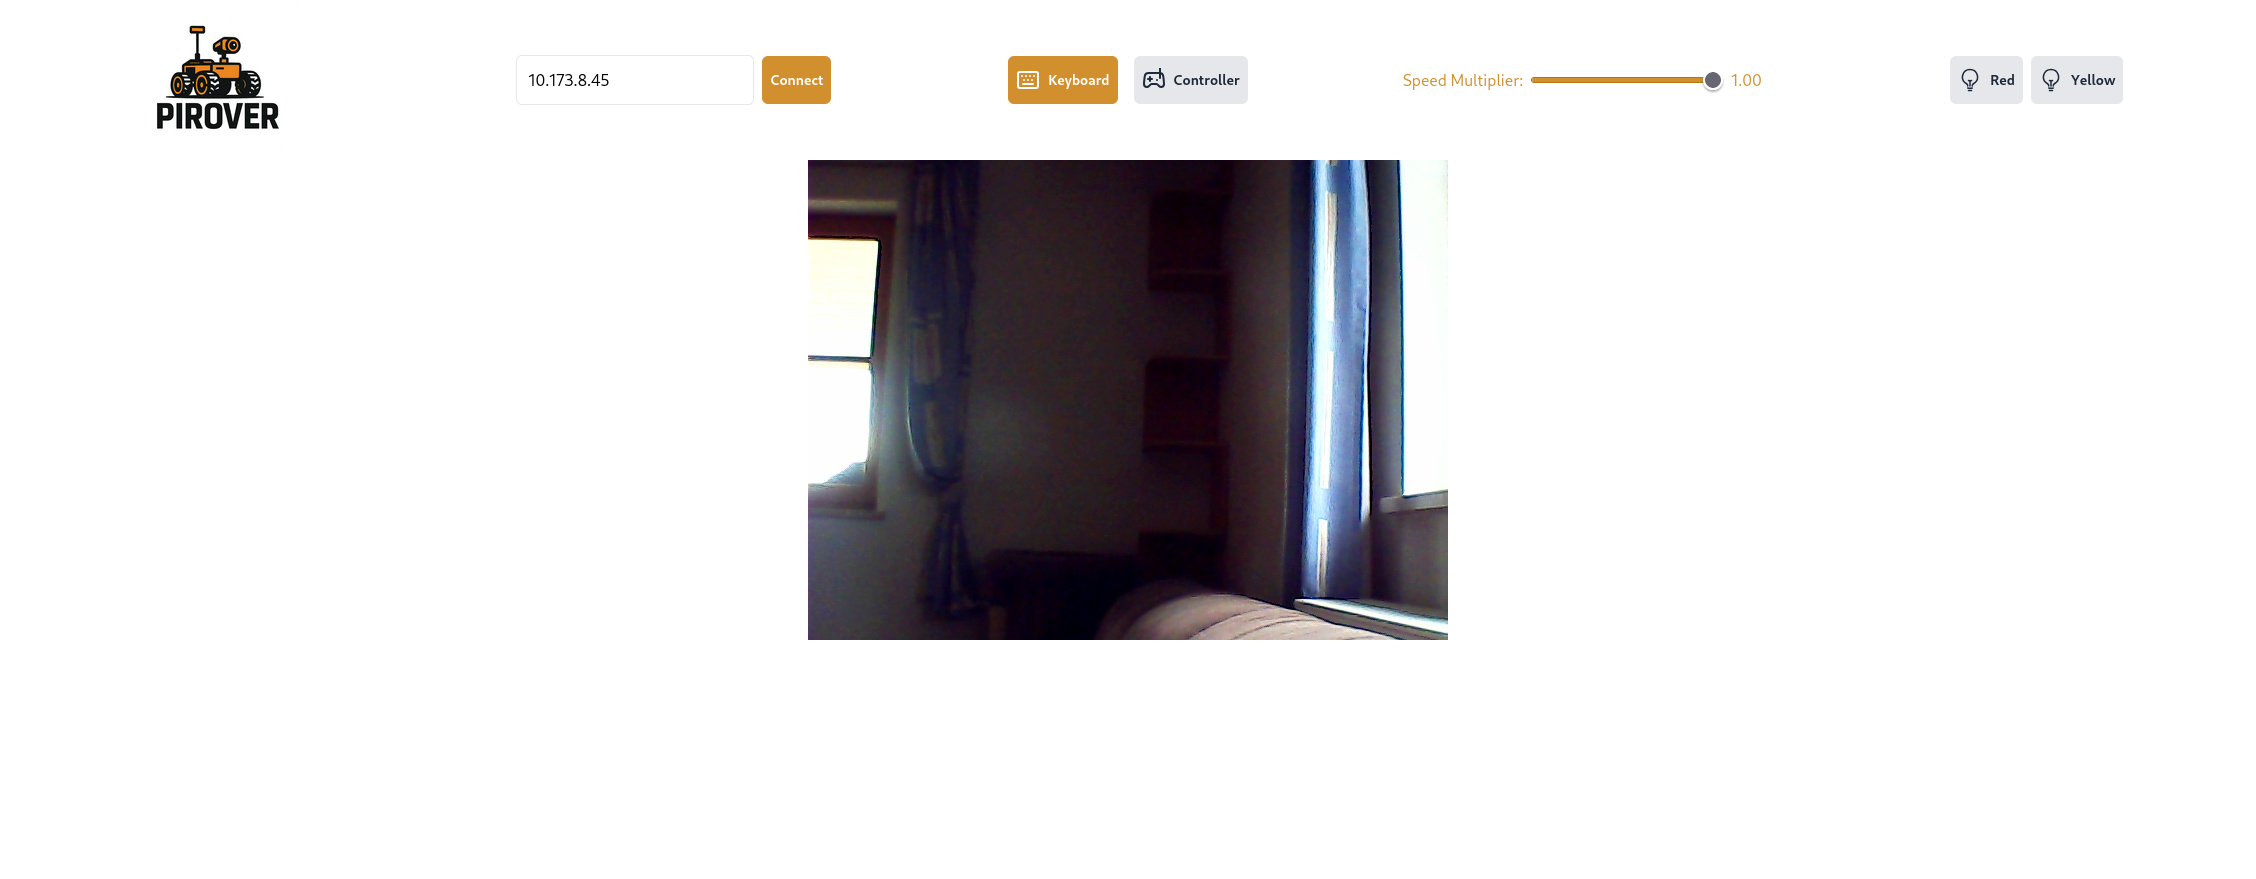
\includegraphics[width=\linewidth]{img/web.png}
\end{figure}

The following controls are available:

\begin{itemize}
    \item driving forwards and backwards
    \item steering the front wheels
    \item making the camera look in a different direction
    \item activating and deactivating the buzzer
    \item activating and deactivating either a red or an orange light
\end{itemize}

The application connects to PiRover via websockets. Tailwind CSS is used to make styling more elegant. In the following, we will examine the critical files and functionalities in more detail, file by file:

\subsection*{\texttt{App.svelte}}

This is the main Svelte component that holds the web application together. It defines an input where you can enter an IP address to connect to PiRover. It also specifies the creation of the websocket connection. Once connected, this file also displays controls for switching between keyboard and gamepad as the input method, buttons to turn PiRover's lights on and off, a slider that can make PiRover go faster or slower and the live camera feed. It also defines the handler functions to send the various controls to PiRover via the websocket connection. To make the application more modular, however, we extracted the functionality to display the live camera feed and to detect inputs into the separate Svelte components \texttt{Camera.svelte} and \texttt{Controls.svelte}.

\subsection*{\texttt{Camera.svelte}}

This file listens to the websocket connection and displays the image if available.

\subsection*{\texttt{Controls.svelte}}

This component primarily defines the buttons to switch between keyboard and gamepad as the input method. These buttons internally either set an instance of the \texttt{keyboard.ts} class or an instance of the \texttt{gamepad.ts} class as the current source. These classes both implement the \texttt{source.ts} interface to make this more elegant. The inputs received from the current source then basically get forwarded to the websocket connection and sent to PiRover.

\subsection*{\texttt{source.ts}}

On the one hand, this interface defines a field \texttt{state} that describes the current state of the input method, like the current camera direction or steering angle. On the other hand, it defines what actions an implementation of the \texttt{Source} interface should notify us about. The implementations \texttt{keyboard.ts} and \texttt{gamepad.ts}  then simply modify the state field and notify us about the interesting inputs according to the specifics of the respective input method.


    \section{Grafana and PostgreSQL}

To provide a clearer overview of the rover's data, we chose Grafana for real-time visualization.
The incoming data from the rover is stored in a PostgreSQL database with the TimeScaleDB extension, which optimizes the handling of time-series data.

Both Grafana and PostgreSQL run directly on the Raspberry Pi using Docker containers.
However, this setup is flexible since the data is transmitted via MQTT, it can easily be reconfigured to run on a separate server.

The database contains a single table, while different sensors and actuators publish their data to distinct MQTT topics. These topics are used to distinguish between data sources.

The rover’s control unit publishes data to the MQTT topic with the format \texttt{rover/sensor\_name}.
A Python script (\texttt{monitoring/mqtt\_to\_postgres.py}) subscribes to these topics and inserts the incoming data into the database.

The Grafana dashboard (\texttt{monitoring/grafana\_dashboard\_templates/data\_dashboard.json}) is configured to query the database and visualize the data, offering a view of the rover’s state.
The specific topics visualized can be seen in the following image:

\begin{figure}[H]
    \centering
    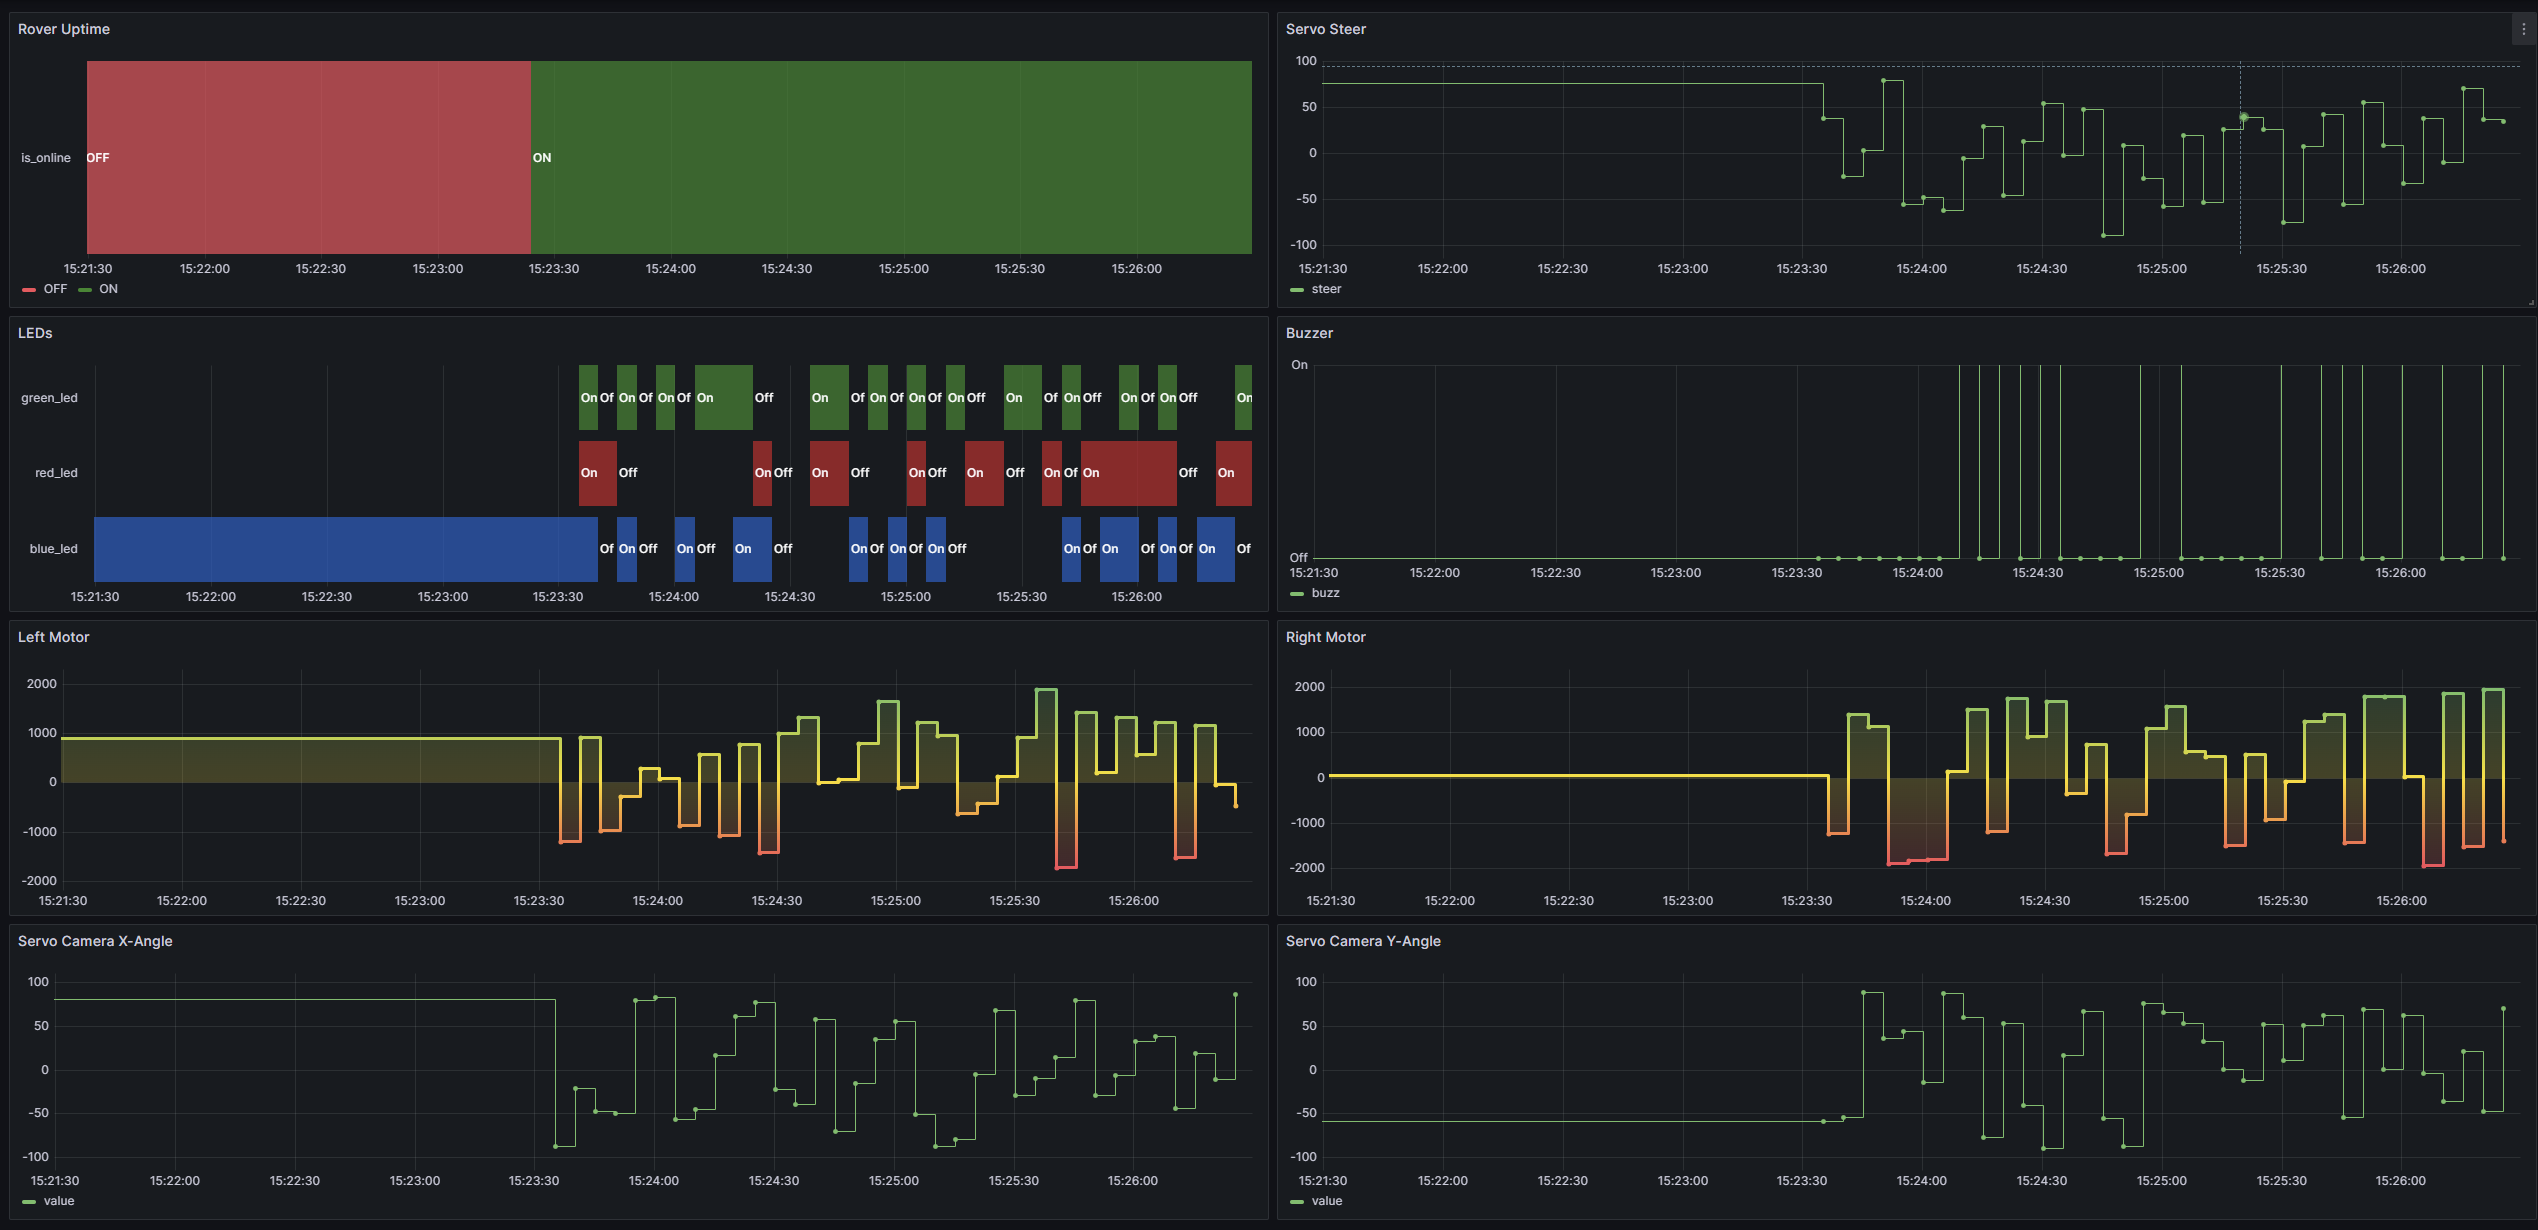
\includegraphics[width=0.95\textwidth]{img/grafana_dashboard}
\end{figure}


    \section{Git Repository}

This is the link to our Git Repository:\\
\href{https://github.com/FabianSchoenberger/PiRover.git}{\textbf{github.com/FabianSchoenberger/PiRover.git}}.

    \section{Problems}

%TODO add more problems

During the course of the project, we encountered several challenges that required us to find practical solutions. The main issues were:

\begin{itemize}
    \item \textbf{Hardware selection and procurement:}
    Since we decided to use a commercial vehicle kit instead of the equipment provided by the institute, we had to handle the procurement ourselves. It took some time to choose a suitable kit, as we first had to verify compatibility with the Raspberry Pi we planned to use. Additionally, finding and ordering the right batteries for power supply required further research. Delays in the delivery of components pushed back our project timeline.

    \item \textbf{Limited testing capabilities:}
    As we only had one Raspberry Pi and one vehicle kit, which were mounted together, testing was limited to one team member at a time. This made it more difficult to verify newly developed software features, as only the person currently in possession of the hardware could run tests. The rest of the team had to rely on that member to verify their work.

    \item \textbf{Power connection issues:}
    The battery holder with the included DC plug, used to power the Raspberry Pi shield, had an intermittent contact issue that was difficult to locate. This caused unexpected power losses and system shutdowns during development and testing, making debugging and progress more difficult.
    \item \textbf{...}
\item \end{itemize}
    \section{Future work}

%TODO Add Possible future work and improvements

In the future, the PiRover can be extended with new hardware and improved functionality. Some possible ideas are:

\begin{itemize}
    \item \textbf{Adding more hardware} \\
    The rover can be equipped with additional components like a second camera on the back (rear view camera) or an ultrasonic distance sensor. These would help with better navigation and safety.

    \item \textbf{Autonomous driving} \\
    The software can be extended to detect lines or paths using the camera. This would allow the rover to drive on its own by following a line on the ground.

    \item \textbf{Improve Grafana Dashboard} \\
    To enhance the user's understanding of the rover's state, the Grafana dashboard could offer a more intuitive interpretation of the data.
    For instance, motor values could be displayed as a percentage of the maximum speed rather than raw numbers.
    Additionally, if the rover shuts down unexpectedly, some data may be lost.
    In such cases, the dashboard might misleadingly show that a component like an LED is still on, simply because it displays the last received state.

\end{itemize}


\end{document}